\documentclass{article}
% Add team performance matrix, schedule to achieve tasks

\usepackage{rob_537}
\usepackage[utf8]{inputenc} % allow utf-8 input
\usepackage[T1]{fontenc}    % use 8-bit T1 fonts
\usepackage{hyperref}       % hyperlinks
\usepackage{url}            % simple URL typesetting
\usepackage{booktabs}       % professional-quality tables
\usepackage{amsfonts}       % blackboard math symbols
\usepackage{nicefrac}       % compact symbols for 1/2, etc.
\usepackage{microtype}      % microtypography
\usepackage{graphicx}       % images
\begin{document}

\title{Learning a Cost Function for Robotic Grasping}
\author{Ammar Kothari, {~} Eddie Taewan Lee, {~} Aisha McKee\\
    Oregon State University \\
    \texttt{\{kotharia, leetae, mckeeai\}@oregonstate.edu}}

\maketitle

\begin{abstract}
% One paragraph "ad" for paper, 1-2 sentence summary of each section
% Final Paper: 1-2 sentences on key results

% Idea first: "In this paper, we introduce...", "The problem is important/critical...", "However, the problem current methods don't work.", "Our approach addresses this...key feature of this approach...", "This helps solve this difficult problem in ...way...", "Our results show..."

% Problem first: "Problem is important...", "However the problem is dificult and current methods don't work...", "In this paper, we...", "Key features of this new approach...", "This helps solve this difficult problem in ...way...", "Our results show..."

    Defining cost functions which describe robotic grasping is challenging. Those cost functions which do exist do not mimic human behavior accurately and conventional analytical models are lacking. In this paper, we use human feedback to train a cost function approximator to improve grasping quality of a two degree-of-freedom reacher. This approach capitalizes upon existing techniques for learned demonstration and incorporates data-driven policy development. This method removes the burden from the developer to define a objective function and allows for human preferences to dominate the technique of the grasping. Our results show a 1000 percent increase in all aspect of grasping. Boo ya!

    We present a cost function for robotic grasping with a two degree-of-freedom reacher, developed using human preferences. This function was compared against automated feedback from a mathematically-derived cost function as well as a controller trained primarily from automated feedback and then slightly modified by human feedback. The OpenAI Reinforcement Learning (RL) Teacher simulator was used during testing to help display and record data. This cost function was modified for use in OpenRAVE to learn a controller to turn various doorknobs through human feedback and validated with SynGrasp, a MATLAB toolbox for grasping.  

\end{abstract}

\section{Introduction}
% Big picture? Difficulties? Significance? Intent of project and its contribution? What's coming in next few paragraphs? 

% Less jargon, why is grasping significant????? Broad audience, cite more of our statements (especially declarative), 2-3x longer! 
% Why is human feedback relevant? Why doesn't everyone use it? "The key contribution of this work is..."

    Grasping is a challenging task for most robots.  In controlled environments -- where everything is known (e.g. position, calibration, point clouds, etc.), the object is fixed, and hand has no compliance -- robots have had some success in grasping an object.  Unfortunately, such a constrained case is unrealistic given the uncertainties associated with friction, contact dynamics, and other factors.  Now, there is a push to reduce these constraints to help mimic the real world and broaden the use of robot grasping for a variety of applications. 
    
    A versatile solution to grasping for autonomous robots does not yet exist.  Using a cost function to train robots is one of the best solutions for successfully grasping objects.  Ideally, the robot can learn while operating; thus, getting more out of an action than simply performing a given, commanded task.  The most basic approach to controlling a robot is to describe a policy in a physical environment that can be used to drive a model to a final stage \cite{byravan2017se3}.  Finding the most optimized behavior value is called the cost function.  
    
    The current state of grasping is fraught with challenges.  Ensuring the gripper is in the correct location poses an initial issue, but is further complicated by potential noise in sensor measurements, changes to material mechanics, and calibration misalignment.  In this work, these problems will be resolved by using human feedback to establish a cost function as a means of assessing the success of a grasping task. 
    
\section{Background} 

\subsection{Grasping}
\subsection{}
% Specifics about problem, key background needed to understand/solve problem, general approaches, related work (literature review, you want it to be strong and compelling as motivation for your solution), what do they do now and why is what you're doing novel?

% More citations, organize by subsections (human feedback, grasping, etc), make sure you have text between sections/subsections/subsubsections, provide context!, don't be too high level 
    
    From path planning to optimized control, learning-based methods have become a staple for solving a variety of robotic problems. Robotic manipulation is no exception; reinforcement learning has been applied to grasping to improve its effectiveness. Random or sporadic movements might be fine for creating successful solutions, but these solutions may not be optimal. Improving repeatability in robotic motion, specifically in robotic manipulation, further improves task repeatability, helps detect failures and recovery modes, and supports interactions with humans\cite{kalakrishnan2013learning}. In order to unlock these benefits, a successful objective function must be developed. In practice this can be quite challenging and often requires manual tuning in order to improve performance of the robot. One solution to this issue is to assume a cost function based on observable trials of a desired, optimal behavior \cite{kalakrishnan2013learning}. Two methods which employ this technique are inverse reinforcement learning (IRL) and inverse optimal control (IOC). The main benefit of using IRL or IOC is that it is generally easier to show what an optimal behavior looks like, rather than trying to develop the mathematical function which encapsulates that behavior. These methods learn to capture the underlying intentions of the task. 

    Even when a grasping task is achieved, the path used often differs from the path chosen by a human subject.  While this is not a limitation on performance, it does lack similarity to human motion.  Additionally, most grasping cost functions simply reward the act of grasping and not the path or method which are used.  By introducing human feedback, the path and final grasp could be improved to reflect human motion better. As of yet, little research has been conducted on developing a cost function for general grasping by means of human feedback. This project seeks to achieve this goal.  Developing a cost function is not easy.  A significant part of modern control is developing an appropriate cost function to embody a task.  This is straightforward for simple tasks like line following or temperature control, but as the complexity of the task increases, it becomes more challenging to accurately capture the cost function.  As a result, cost functions are commonly seen as arbitrary solutions to the problem.  Another method for defining cost functions is to derive it from examples of good and bad actions.  These examples can be provided by another algorithm or, potentially, a person.  With a human, the cost function will encode their preferences.  This is especially powerful when we can identify a behavior but cannot define an analytically combination of states that rewards that behavior.  Additionally, this allows a non-expert user to program complex tasks through feedback.

\subsection{Inverse Reinforcement Learning}

    The idea of using human feedback to program is part of a new branch of programming.  With machine learning, a computer can generate and modify programs to meet user expectations.  This ideology departs from the classical notion of programming where an expert user is required to carefully assemble lines of code.  The feedback based style is known as Interactive Learning and Optimization (ILO)\cite{Akrour2014}.  Inverse Reinforcement Learning (IRL) is captured in this classification.
    
    Kalakrishman et al. present a method for establishing an objective function based on IRL. This method has been applied directly to redundancy in inverse kinematics as well as optimized motion planning for tasks such as grasping or manipulation. The algorithm is based on samples from the region closest to the optimal trajectory, thus helping to make it applicable in higher-dimensional spaces \cite{kalakrishnan2013learning}. During testing, multiple configurations for grasping an object were demonstrated for the robot arm. The object itself was independent of the trial because the goal of the trials was to meet a desired end effector pose. This technique was later applied to motion planning for the robotic arm. Building upon sampling-based motion planning algorithms which create feasible but not optimal paths, this method can additionally consider minimizing other costs such as torque loading, smoothness of path, and other constraints. Using this technique, a cost function for the task can be determined\cite{kalakrishnan2013learning}. Because no ideal cost function of the corresponding human behavior is available, a series of weights were used with IRL to minimize the cost trajectories. 
    
    One way people provide a sense of a task to each other is to demonstrate it. The same strategy can be used with robots.  Using either sensory input or joint angles, a complex task like robotic motion control can be learned from kinesthetic demonstrations\cite{Finn2016}.  \cite{Finn2016} were able to train a robot to complete the task of putting a plate into a dish rack with less than 30 demonstrations.  They utilize a framework where the IRL algorithm (Guided Policy Search \cite{levine2015learning}) provides guidance to the RL algorithm for which trajectories to sample. This has the benefit of keeping new trajectories from deviating too far from old trajectories as well as minimizing the number of iterations required to converge.  Optimizing the cost function separately from the policy can require a significant number of trials for the RL algorithm to converge. \cite{Finn2016} showed that domain knowledge specific regularizers can be used to improve the resulting cost function.  In our work, we will use similar regularizers on the network to increase convexity of the search space. One challenge is that cost functions do not generalize well to other tasks\cite{Finn2016}.  However, the resulting policy does.  The cost function can be more general by presenting enough demonstrations on a variety of tasks to ensure overfitting does not occur to any individual task.
    
    Kinesthetic examples are helpful, but in some cases cannot be provided, especially for robots.  For example, providing kinesthetic examples for running is very difficult.  Instead, finding a different method of providing guidance is important.  This can be done with controllers mapped to joint angles of the robot\cite{mericcli2010biped, DAgger}.  One disadvantage of this approach is that the burden is on the person to provide error corrections to the robot which can be difficult for robot kinematics that are different from our own or for non-humanoid robots like quadcopters.  An alternative is for the algorithm to accept preference.  Gathering the data can be viewed as an interface challenge for Human Robot Interaction, but the goal is to understand how trajectories compare to each other to better estimate the underlying cost function\cite{Akrour2014,  Christiano2017}.  This reduces the burden of feedback while still providing sufficient information to adjust the cost function.
    
    When using preference comparison, complex tasks have been taught to a robot in simulation\cite{Christiano2017}.  The goal is to minimize the amount of feedback required while maximizing the performance of the reinforcement learning algorithm.  Receiving less than 1\% of interactions is still sufficient to learn a task\cite{Christiano2017}.  Feedback is least impactful at the beginning of learning when all attempts are equally bad and at the end when the expert begins to make mistakes because performance is sufficiently good\cite{Akrour2014}.  Specific RL algorithms are required to be successful with IRL.  Only those that are capable of handling non-stationary cost functions will be able to interact with IRL.  Methods that degrade significantly with changes to the cost function will require increased time to converge after every cost function update.  Although this does not change the amount of feedback required, the amount of time required to learn a task increases significantly.
    
    It is generally assumed when doing motion planning that all objects and poses are known accurately. Yet, uncertainty can be one of the main issues facing robotic manipulation. Humans can easily adapt grasping trajectories given state estimation uncertainty, thus yielding better force-closure performance. Stulp et al. propose a method for learning motion which is robust to uncertainties in the state estimation \cite{stulp2011learning}. Reaching and preshaping together are used to improve the likelihood that the grasp will succeed, as compared to each being evaluated independently in an environment where perfect knowledge of all the poses is known. Using a distribution of poses which incorporate uncertainty of the state, the arm looks to grasp the object from this distribution rather than a single, known pose \cite{stulp2011learning}.

    Learning-based control is relatively new to robot grasping and the full capability has not been uncovered yet.  This shift is partially due to the fact that neural networks allow for better function approximation than a regressive or analytical model alone, but also previous approaches have had little success.  Some previous literature has proposed a guided policy search which completes a task by only giving the robot a goal \cite{levine2015learning}, an optimal grasp metric given a depth image \cite{johns2016deep}, and a complete policy which takes in visual data and outputs a motor control \cite{gu2016deep}.  Other methods have included features of the domain (e.g. rigid body motion) in the structure of the network in order to improve estimation \cite{byravan2017se3}.  Many of these works focus on simple tasks for which a cost function could be fully defined.  As a result, the learned actions are quite simple.  Instead, if a complex cost function can be defined, these methods should also be able to learn complex tasks.  This project will build upon the previous approaches by attempting to learn a cost function directly from human feedback.

\section{Method}
% What is your solution? Describe algorithm/theory (programs/simulators you use)

% Not "method" or "simulation" actually use name of algorithm

    We will conduct initial testing in the OpenAI Gym environment for a 2D-reacher.  This environment will demonstrate many of the challenges of our project in a much simpler domain.  We will test out our IRL function approximator in this environment.  Additionally, we will use a Trust Region Policy Optimization (TRPO) \cite{SchulmanLMJA15} for our RL algorithm to couple with our IRL implementation.  The TRPO algorithm stably improves performance and can handle changes in the cost function \cite{Christiano2017}.  We may explore other methods that also rely on trust regions and are more data efficient as this will reduce time needed and amount of feedback necessary for convergence. When implementing the IRL, an important aspect to understand is the amount of feedback required and how much can be synthetic (i.e. from a hand designed cost function) and how much should be provided by people.  We will implement our feedback system in a simulator using code from \cite{Christiano2017}.  This framework will allow us to easily display and record feedback.  Given the popularity of OpenAI's platform, a lot of the code should be available, but has not yet been combined in the way we envision.

	Once we have settled on an implementation, we will transition to an environment like OpenRAVE that is more amenable to grasping.  The goal task is to grab a handle and rotate it.  We will use state information with injected noise as the input to our model.  We will teach a controller with automated feedback from a cost function we conceive. We will also train a controller from only human feedback.  Finally, we will train a controller primarily from automated feedback, and then change the behavior slightly using human feedback.  The task is complex enough to show the usefulness of the approach, as well as understand the amount of human feedback that is necessary to learn complex cost functions.
	
	As a final step, we will work with SynGrasp, a MATLAB toolbox designed specifically for grasping analysis of human and robotic hands \cite{malvezzi2015syngrasp}. SynGrasp allows for the analysis and visualization of many of the main grasp properties (e.g. forces, motions, manipulability, etc.). It also allows for the assessment of individual limbs and joints in the grasping gesture as well as the implementation of limits on certain components to accurately reflect the robot hand model. SynGrasp has an automated grasp planner which allows for comparison with the grasping cost function \cite{malvezzi2013syngrasp}. This grasp planner takes in the reacher model, object, number of pregrasp positions, and metric for evaluation and returns the best grasp from simulation \cite{malvezzi2015syngrasp}. All other grasps tested during the trial can also be accessed in the simulator. 
	
\section{Results}
% Describe set of experiments you conducted, preliminary results
% Final Paper: detailed results, analysis of results
%!TEX root = PreliminaryPaper.tex
\subsection{Toy Domain}
Toy domain is two degree of freedom reacher from Mujoco.

\subsubsection{Synthetic Data}
\begin{figure}[h]
    \centering
    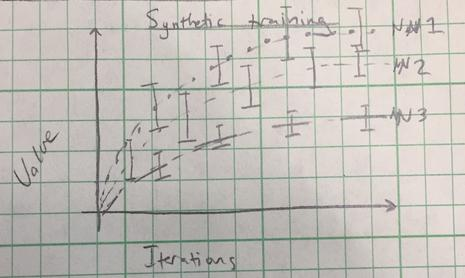
\includegraphics[width=0.9\textwidth]{Images/ToySyntheticTrainingAccuracy.jpg}
    \caption{Training progress of cost function}
    \label{fig:ToySyntheticTraningAccuracy}
\end{figure}

\begin{figure}[h]
    \centering
    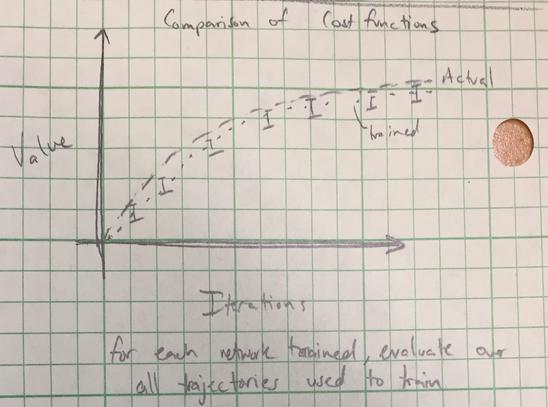
\includegraphics[width=0.9\textwidth]{Images/ToySyntheticCostComparison.jpg}
    \caption{Comparison of trained cost function to actual cost function.}
    \label{fig:ToySyntheticCostComparison}
\end{figure}

\begin{figure}[h]
    \centering
    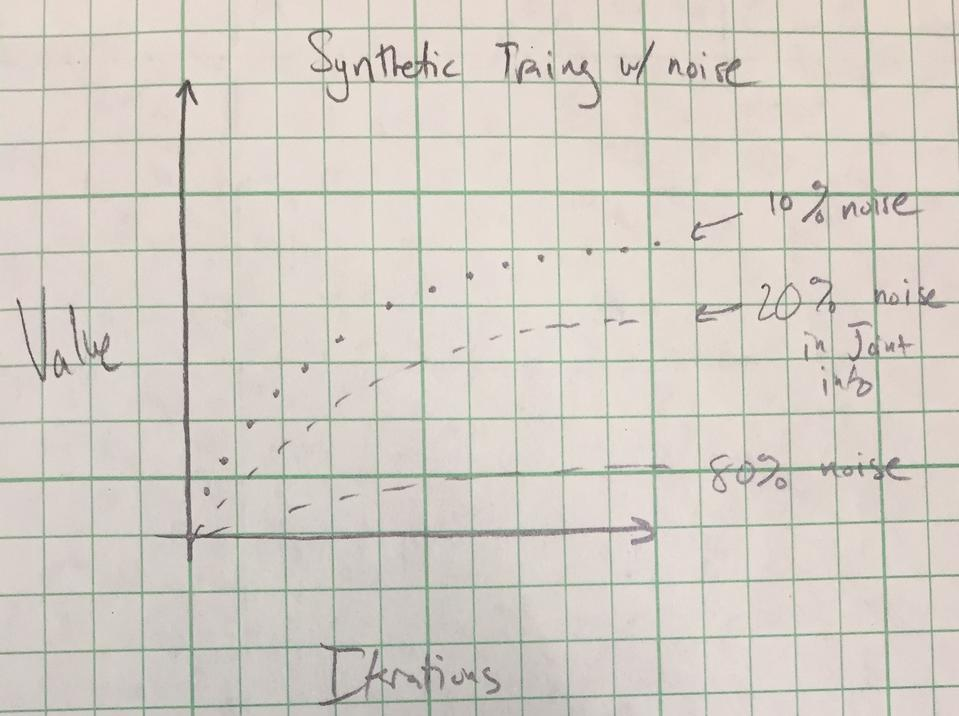
\includegraphics[width=0.9\textwidth]{Images/ToySyntheticNoise.jpg}
    \caption{Comparison of trained cost functions with different amounts of noise.}
    \label{fig:ToySyntheticNoise}
\end{figure}

\subsection{Human Training}

\begin{figure}[h]
    \centering
    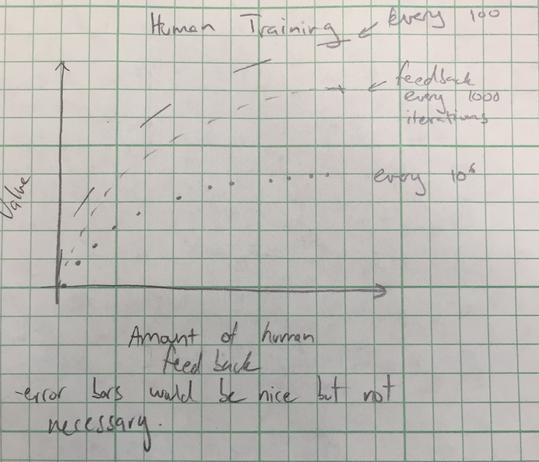
\includegraphics[width=0.9\textwidth]{Images/ToyHumanTrainingProgress.jpg}
    \caption{Training progress of cost function with human feedback.}
    \label{fig:ToyHumanTraningProgress}
\end{figure}

\begin{figure}[h]
    \centering
    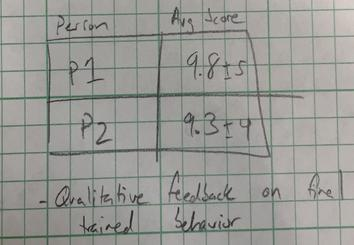
\includegraphics[width=0.9\textwidth]{Images/ToyHumanCostComparison.jpg}
    \caption{Qualitative estimate of how much a person agrees with the goal behavior.}
    \label{fig:ToyHumanCostComparison}
\end{figure}


\subsection{Combined Training}
\begin{figure}[h]
    \centering
    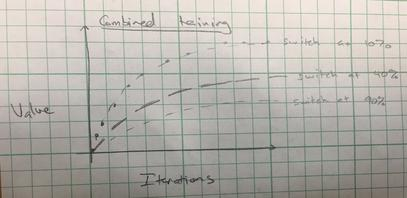
\includegraphics[width=0.9\textwidth]{Images/ToyCombinedTraining.jpg}
    \caption{Training progress of cost function with synthetic feedback followed by human feedback.}
    \label{fig:ToyCombinedTraningProgress}
\end{figure}


\subsection{Grasping Domain}
Grasping domain is turning a handle.  Software used is OpenRAVE.  Ported over same framework.

\begin{figure}[h]
    \centering
    
\includegraphics[width=0.25\textwidth]{Images/placeholder.png}
    \caption{Training progress of cost function}
    \label{fig:GraspingSyntheticTraningAccuracy}
\end{figure}

\begin{figure}[h]
    \centering
    
\includegraphics[width=0.25\textwidth]{Images/placeholder.png}
    \caption{Training progress of cost function}
    \label{fig:GraspingCombininedTraningProgress}
\end{figure}





\section{Discussion and Conclusion}
% Key contributions of paper, key insights, future work
% Able to repeat content from abstract (assuming it's tight)

\section{Acknowledgments}

\section{References}

\medskip
\small

\bibliographystyle{unsrt}
\bibliography{AllPapers}

\end{document}


    % papers
    % \begin{itemize}
    %     \item demonstration
    %     \item current status in robotic grasping
    %     \item openAI paper overview -- synthetic vs. human feedback -- 
    %     \item degeneracy in cost functions
    %     \item 
        
    % \end{itemize}